%%%%%%%%%%%%%%%%%%%%%%%%%%%%%%%%%%%%%%%%%
% baposter Portrait Poster
% LaTeX Template
% Version 1.0 (15/5/13)
%
% Created by:
% Brian Amberg (baposter@brian-amberg.de)
%
% This template has been downloaded from:
% http://www.LaTeXTemplates.com
%
% License:
% CC BY-NC-SA 3.0 (http://creativecommons.org/licenses/by-nc-sa/3.0/)
%
%%%%%%%%%%%%%%%%%%%%%%%%%%%%%%%%%%%%%%%%%

%----------------------------------------------------------------------------------------
%	PACKAGES AND OTHER DOCUMENT CONFIGURATIONS
%----------------------------------------------------------------------------------------

\documentclass[a0paper,landscape]{baposter}

\usepackage[export]{adjustbox}
\usepackage{graphicx}

\usepackage[font=small,labelfont=bf]{caption} % Required for specifying captions to tables and figures
\usepackage{booktabs} % Horizontal rules in tables
\usepackage{relsize} % Used for making text smaller in some places

\graphicspath{{figures/}} % Directory in which figures are stored

\definecolor{bordercol}{RGB}{40,40,40} % Border color of content boxes
\definecolor{headercol1}{RGB}{186,215,230} % Background color for the header in the content boxes (left side)
\definecolor{headercol2}{RGB}{80,80,80} % Background color for the header in the content boxes (right side)
\definecolor{headerfontcol}{RGB}{0,0,0} % Text color for the header text in the content boxes
\definecolor{boxcolor}{RGB}{186,215,230} % Background color for the content in the content boxes

\begin{document}

\background{ % Set the background to an image (background.pdf)
\begin{tikzpicture}[remember picture,overlay]
\draw (current page.north west)+(-2em,2em) node[anchor=north west]
{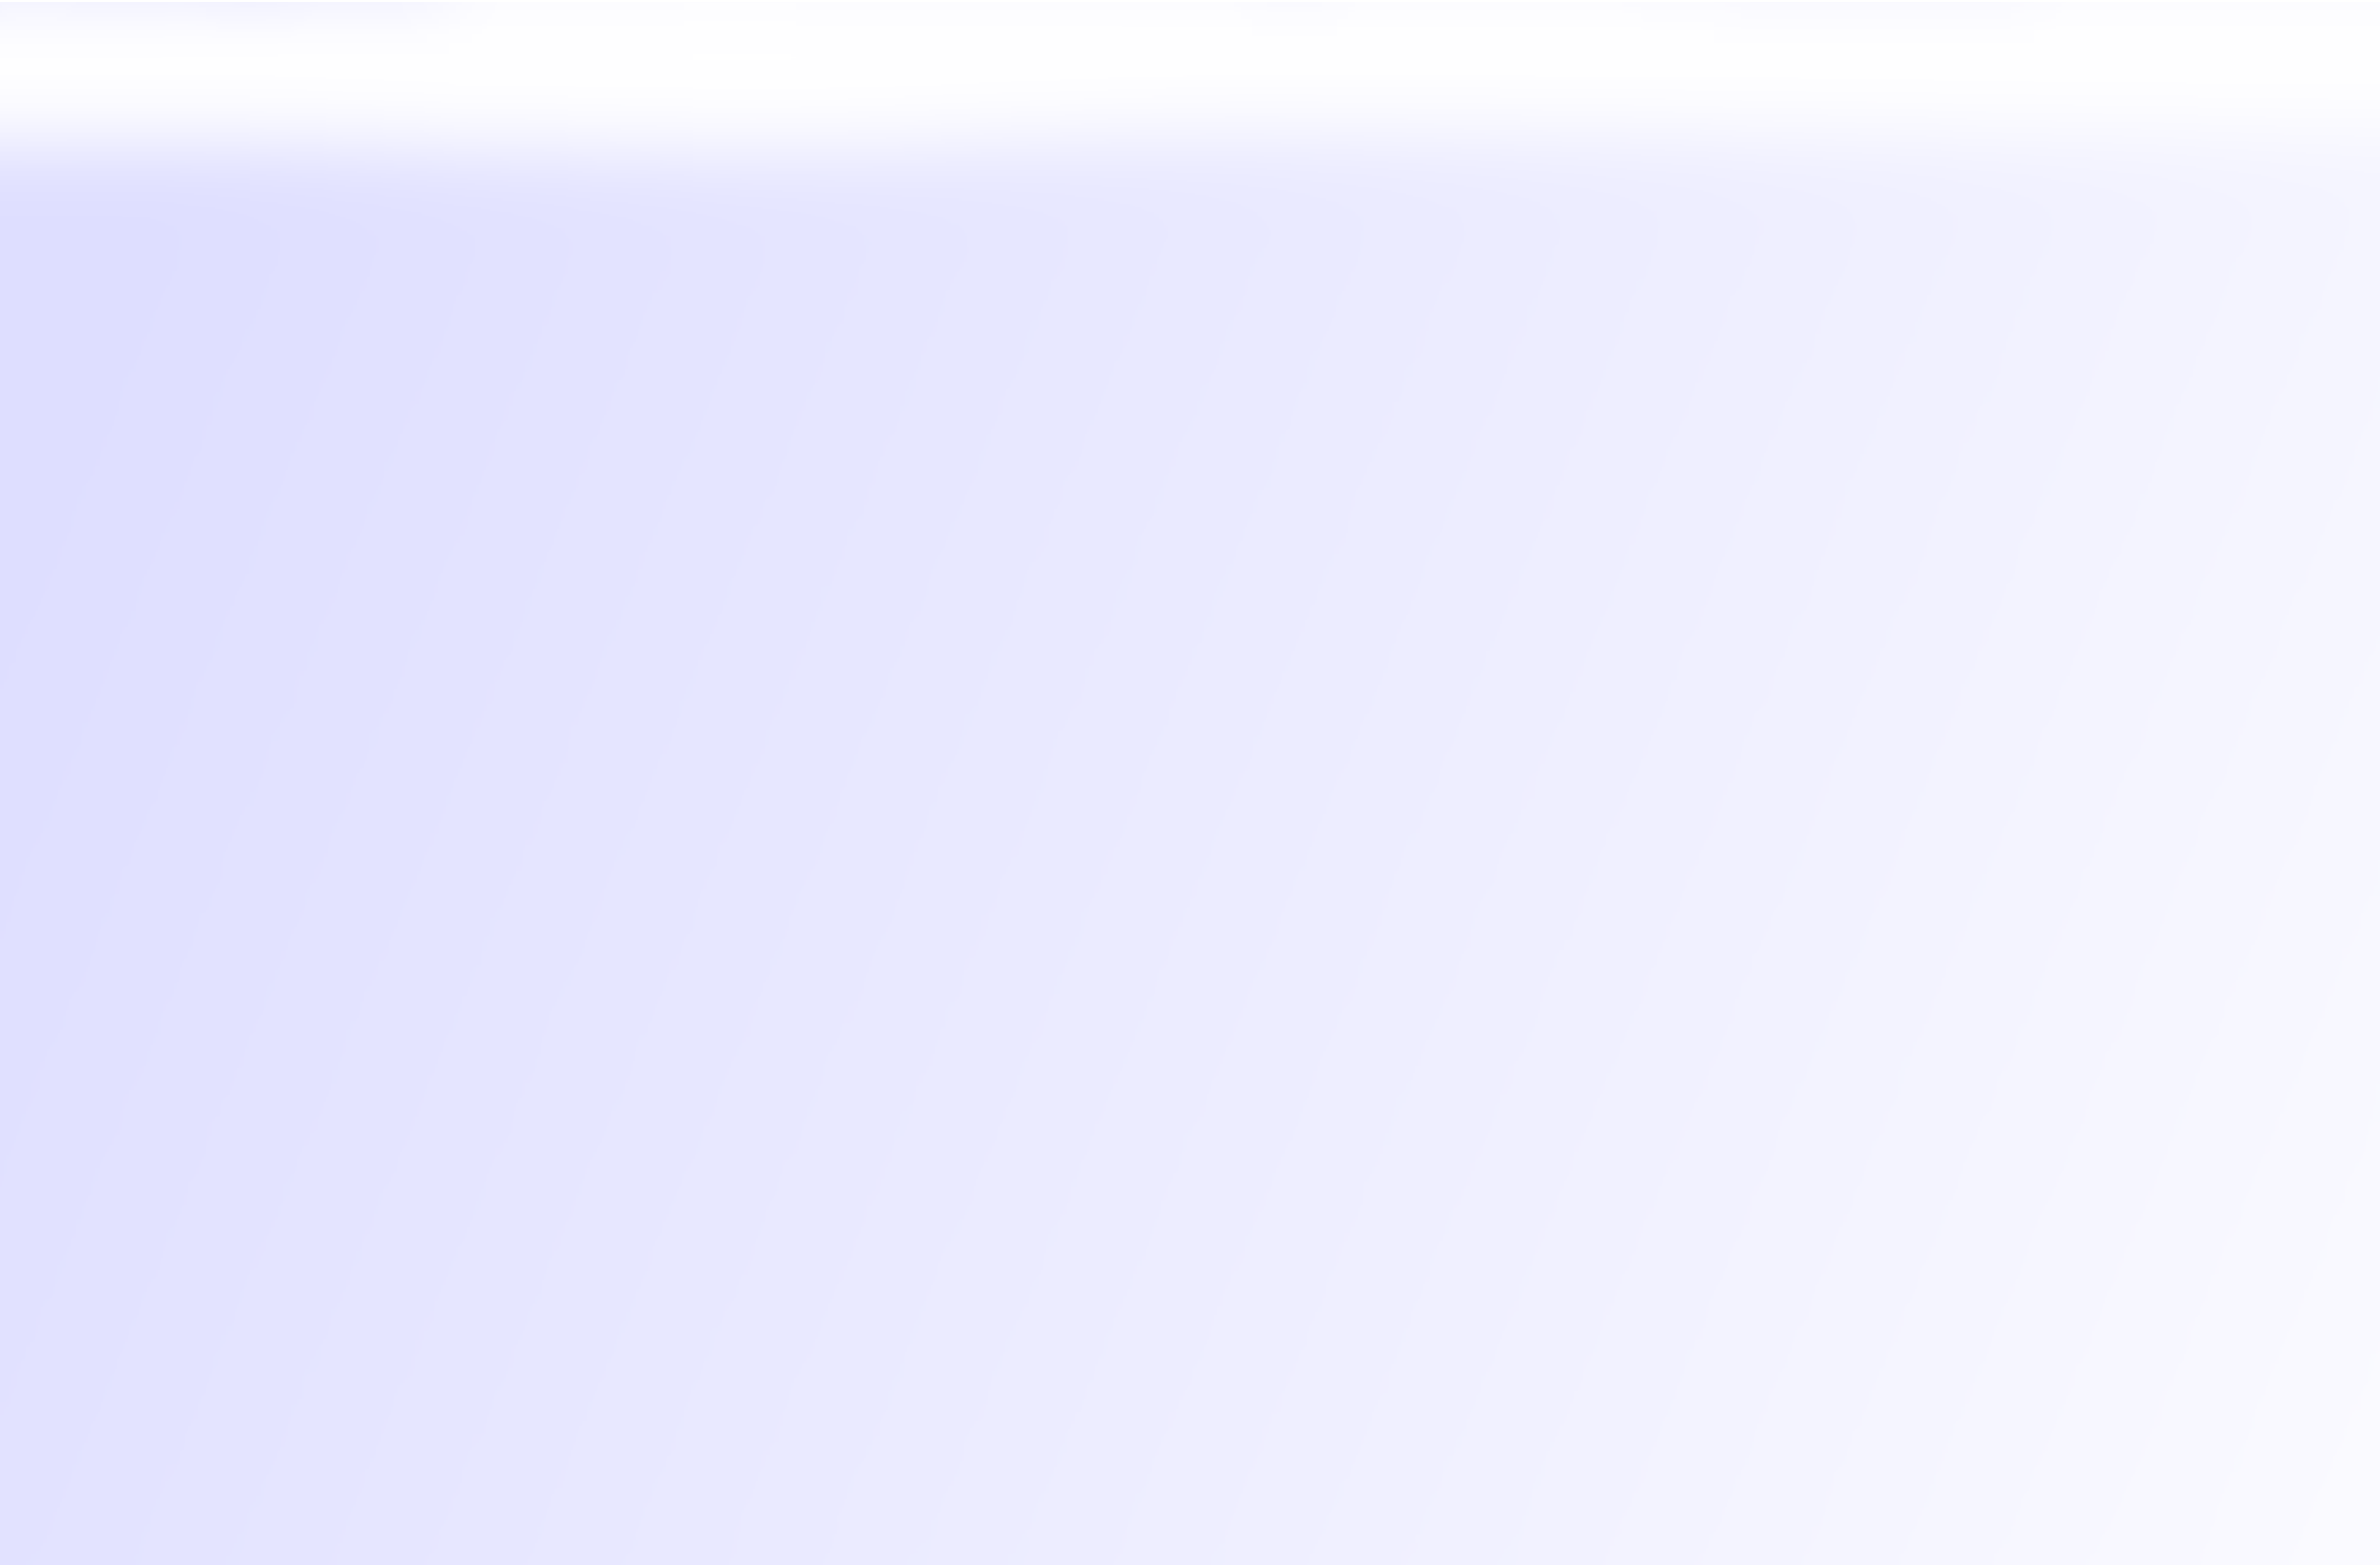
\includegraphics[height=1.1\textheight]{background}};
\end{tikzpicture}
}

\begin{poster}{
grid=false,
borderColor=bordercol, % Border color of content boxes
headerColorOne=headercol1, % Background color for the header in the content boxes (left side)
headerColorTwo=headercol2, % Background color for the header in the content boxes (right side)
headerFontColor=headerfontcol, % Text color for the header text in the content boxes
boxColorOne=boxcolor, % Background color for the content in the content boxes
headershape=roundedright, % Specify the rounded corner in the content box headers
headerfont=\Large\sf\bf, % Font modifiers for the text in the content box headers
textborder=rectangle,
background=user,
headerborder=open, % Change to closed for a line under the content box headers
boxshade=plain
}
{}
%
%----------------------------------------------------------------------------------------
%	TITLE AND AUTHOR NAME
%----------------------------------------------------------------------------------------
%
{\sf\bf\LARGE Characterizing Dislocation Defects in Dark Field X-ray Microscopy Images of Bulk Aluminum} % Poster title
{\vspace{.5em}\smaller Marylesa Howard$^1$, Arnulfo Gonzalez$^1$, Ryan Coffee$^2$, Malena Espa�ol$^3$, Michael Brennan$^4$, Jessica Pillow$^{1,5}$, Eric Machorro$^6$,\\ Eric Clarkson$^5$, Sean Breckling$^1$, Margaret Lund$^1$, Jesse Adams$^1$, Leora Dresselhaus-Cooper$^7$ \\ % Author names
{\scriptsize $^1$Nevada National Security Site, $^2$SLAC National Accelerator Laboratory, $^3$Arizona State University, $^4$Massachusetts Institute of Technology, $^5$University of Arizona, $^6$Pacific Northwest National Laboratory, $^7$Lawrence Livermore National Laboratory}} % Author email addresses
{
\includegraphics[scale=0.25]{nnss_site}}%\hspace{.25in}
\includegraphics[scale=0.4]{llnl}
%
\includegraphics[scale=0.25]{slac}\hspace{.25in}
\includegraphics[scale=0.25]{pnnl}\\
%
\includegraphics[scale=0.25]{asu}\hspace{.15in}
\includegraphics[scale=0.25]{ua}\hspace{.15in}
\includegraphics[scale=0.25]{mit}}
%{
\includegraphics[scale=0.15]{logo}} % University/lab logo

%----------------------------------------------------------------------------------------
%	Abstract
%----------------------------------------------------------------------------------------

\headerbox{Abstract}{name=abstract,column=0,row=0}{
Material defects play a large role in material response under shock loading, yet our understanding of how these defects initiate, propagate, and annihilate are not well understood. Using a newly developed diagnostic, dark field X-ray microscopy (DFXM), we can now visualize the behavior of dislocation defects in materials at the mesoscale under varying conditions. Using data from the European Synchrotron Radiation Facility, we apply a variety of image processing techniques to capture relevant features to locate and characterize size and orientation of dislocation defects in bulk aluminum DFXM images. Beyond simple visualization, this analysis drives statistical characterization of the defects and their dynamic response to further improve the relevant physics models.

}

%----------------------------------------------------------------------------------------
%	DFXM
%----------------------------------------------------------------------------------------

\headerbox{Dark Field X-ray Microscopy}{name=DFXM,column=0,below=abstract, above=bottom}{

Strong shock waves rapidly push materials beyond their yield stress, causing ultrafast plastic deformations forcing the material to exotic transformations and failure.

\begin{center}
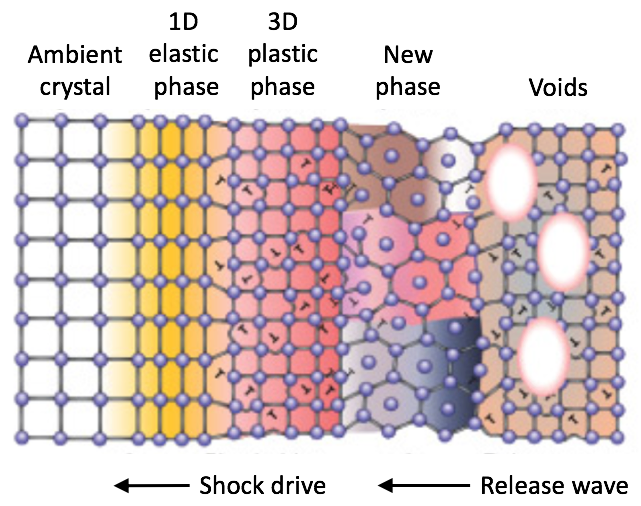
\includegraphics[width=.75\textwidth]{PhaseDiagram}
\end{center}

Detailed mechanisms underlying the onset of plasticity and the resulting deformations are not well understood, and ultrafast dark field X-ray microscopy (DFXM) is a novel imaging technique in development to capture how defects initiate large-scale deformations in materials. 

\begin{center}
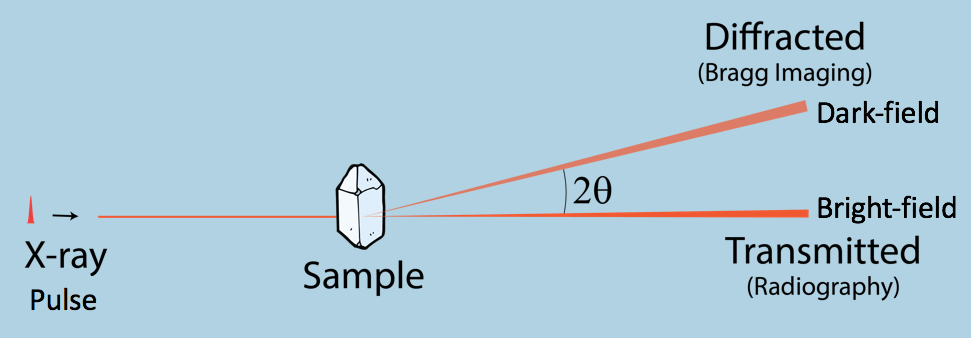
\includegraphics[width=.9\textwidth]{DFXM}
\end{center}
}






%----------------------------------------------------------------------------------------
%	EXPERIMENT
%----------------------------------------------------------------------------------------

\headerbox{Experiments at European Synchrotron Radiation Facility (ESRF)}{name=experiments,span=3,column=1,row=0}{ % To reduce this block to 1 column width, remove 'span=2'


At ESRF, dark field X-ray microscopy images were taken on bulk aluminum. Dislocation defects, a type of plane defect, are present in the data collected and present as paired dark/bright regions in the images. In the images below, sequenced in time, a dislocation inserts into a dislocation boundary.

\begin{center}
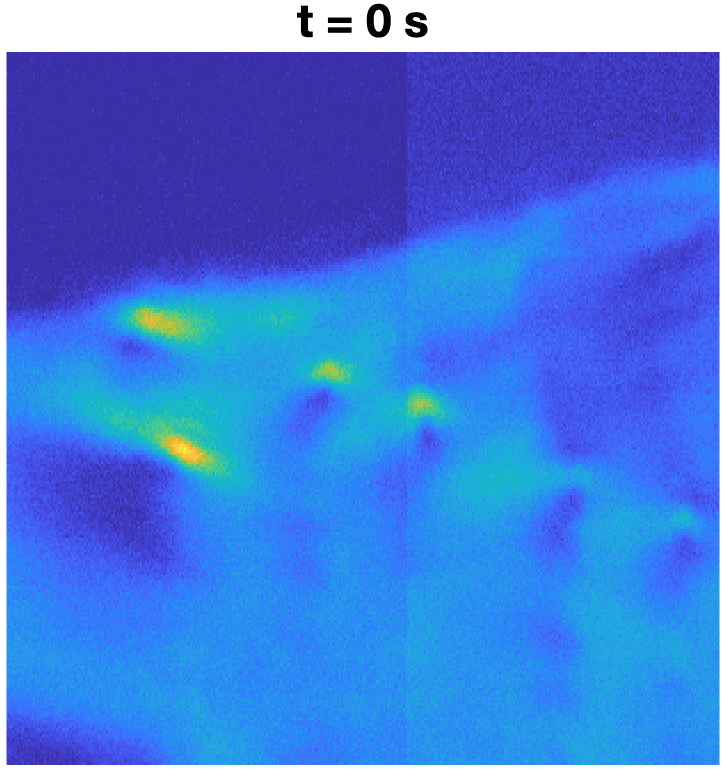
\includegraphics[width=0.1\linewidth]{DisInsert1}\hfill
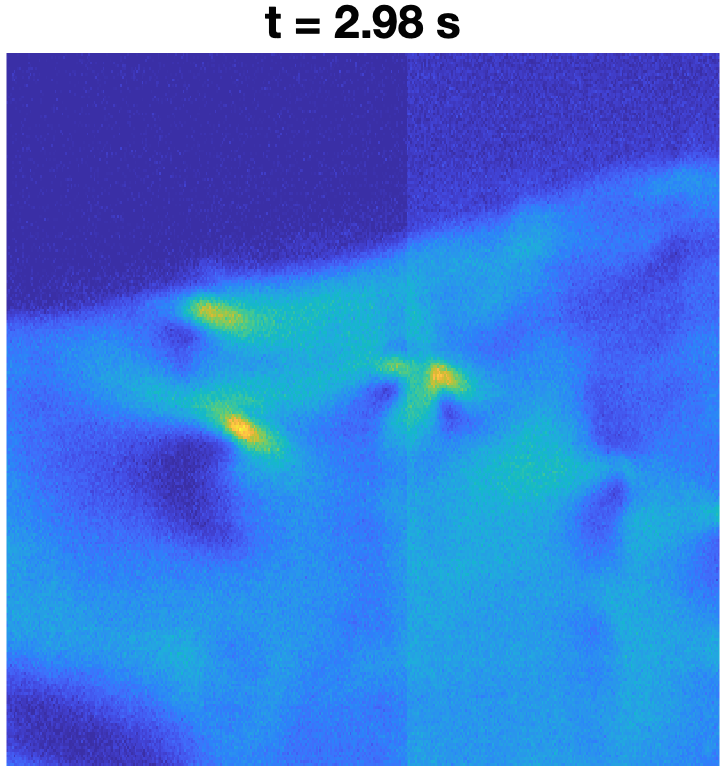
\includegraphics[width=0.1\linewidth]{DisInsert2}\hfill
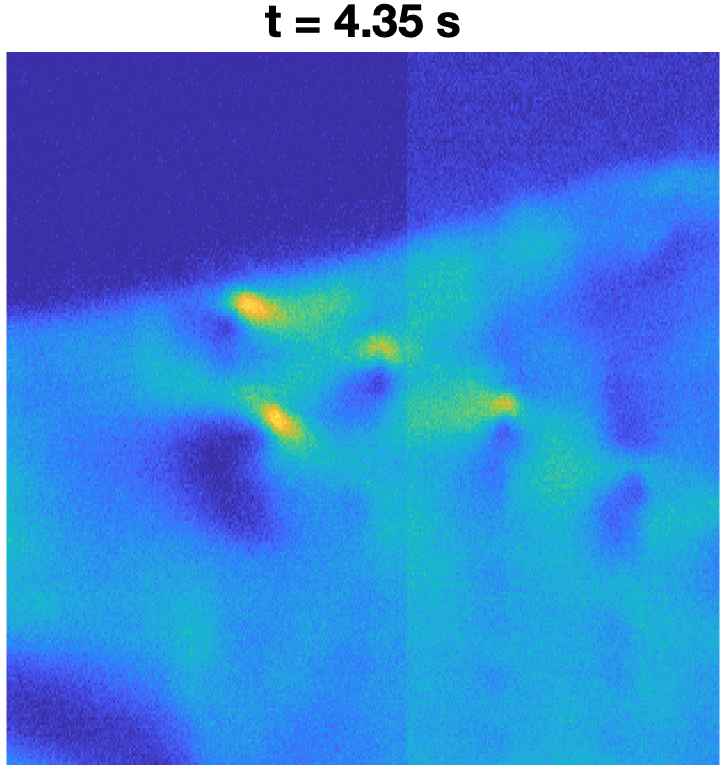
\includegraphics[width=0.1\linewidth]{DisInsert3}\hfill
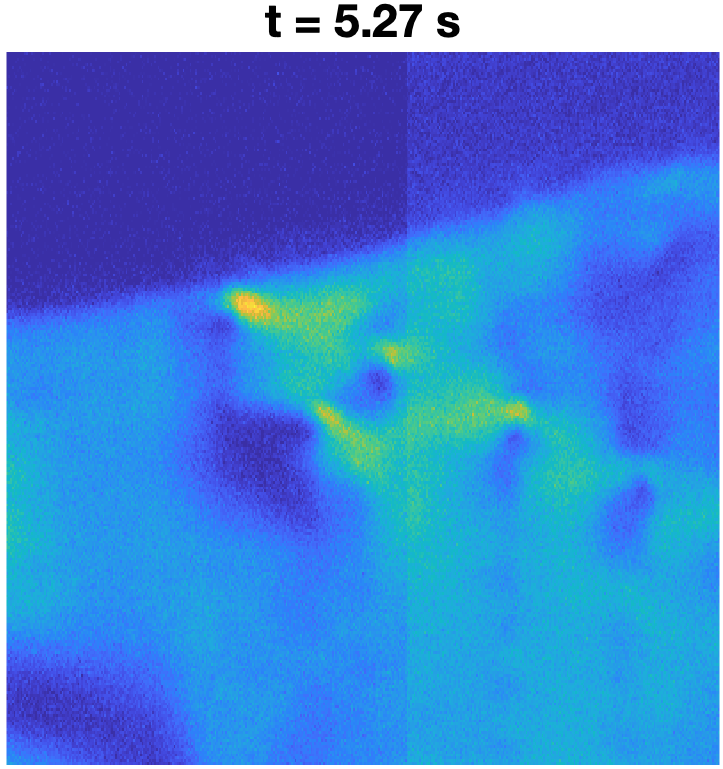
\includegraphics[width=0.1\linewidth]{DisInsert4}\hfill
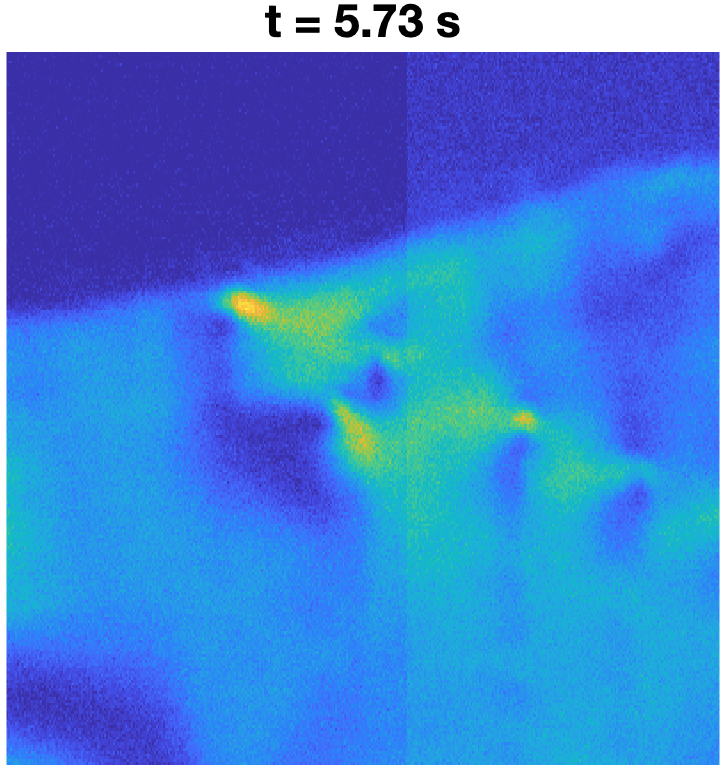
\includegraphics[width=0.1\linewidth]{DisInsert5}\hfill
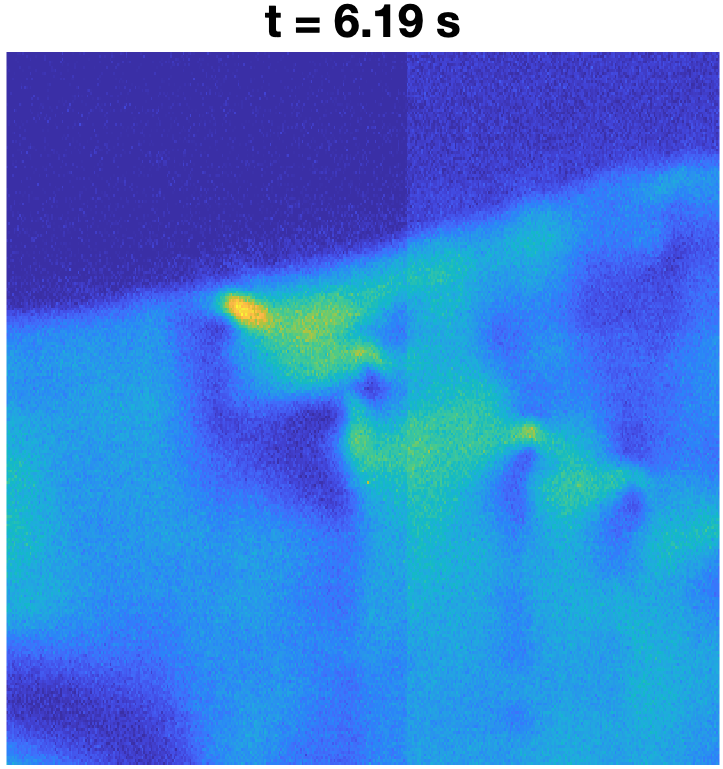
\includegraphics[width=0.1\linewidth]{DisInsert6}\hfill
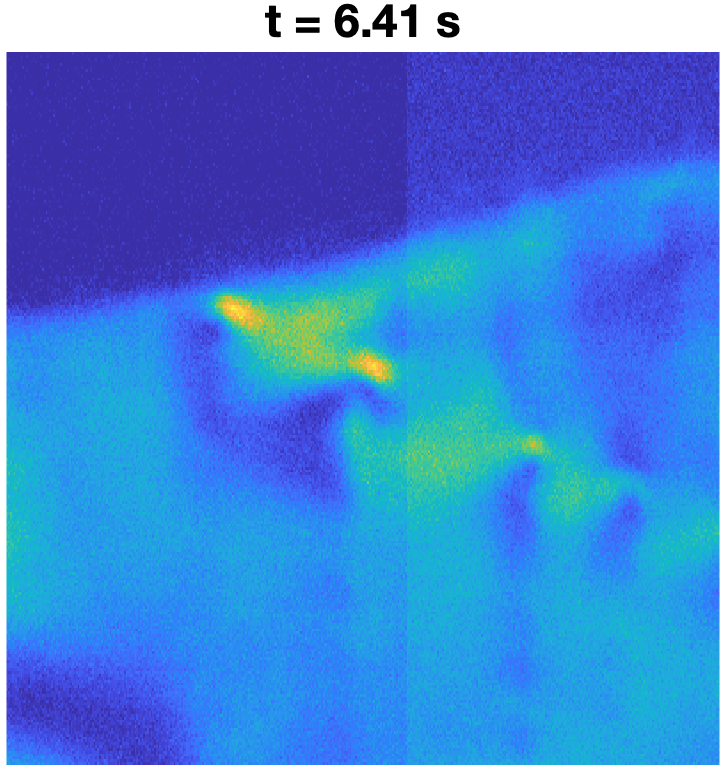
\includegraphics[width=0.1\linewidth]{DisInsert7}\hfill
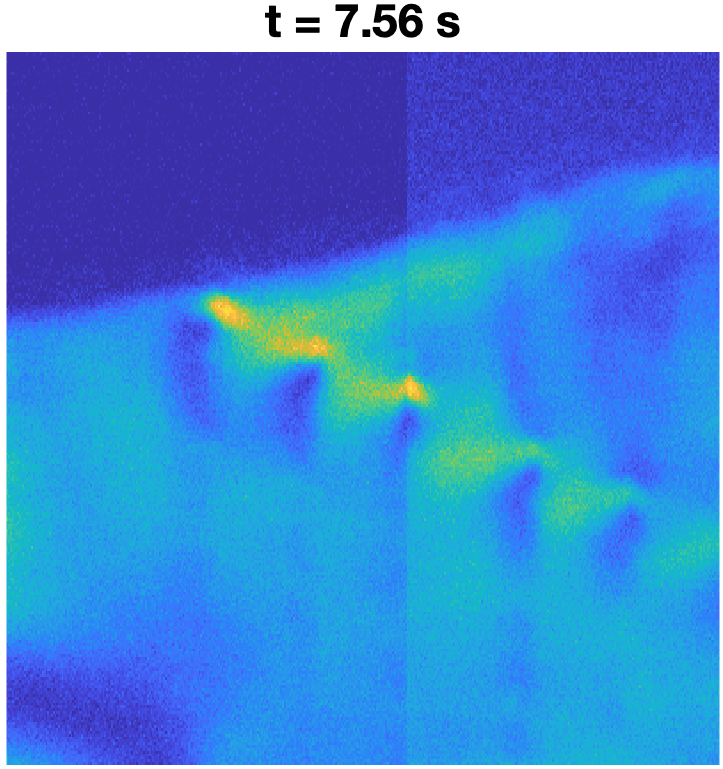
\includegraphics[width=0.1\linewidth]{DisInsert8}
\end{center}
%\captionof{figure}{Figure caption}
%\label{fig:dislocationInsertion}}

Identifying dislocations and relevant statistics through image processing is essential to informing physics models.
}

%----------------------------------------------------------------------------------------
%	IMAGE PROCESSING
%----------------------------------------------------------------------------------------

\headerbox{Image Processing Techniques}{name=imageprocessing,span=2,column=1,below=experiments,above=bottom}{ % To reduce this block to 1 column width, remove 'span=2'

%------------------------------------------------

\noindent
{\begin{minipage}[t]{0.48\linewidth}
\begin{center}
{\hfill
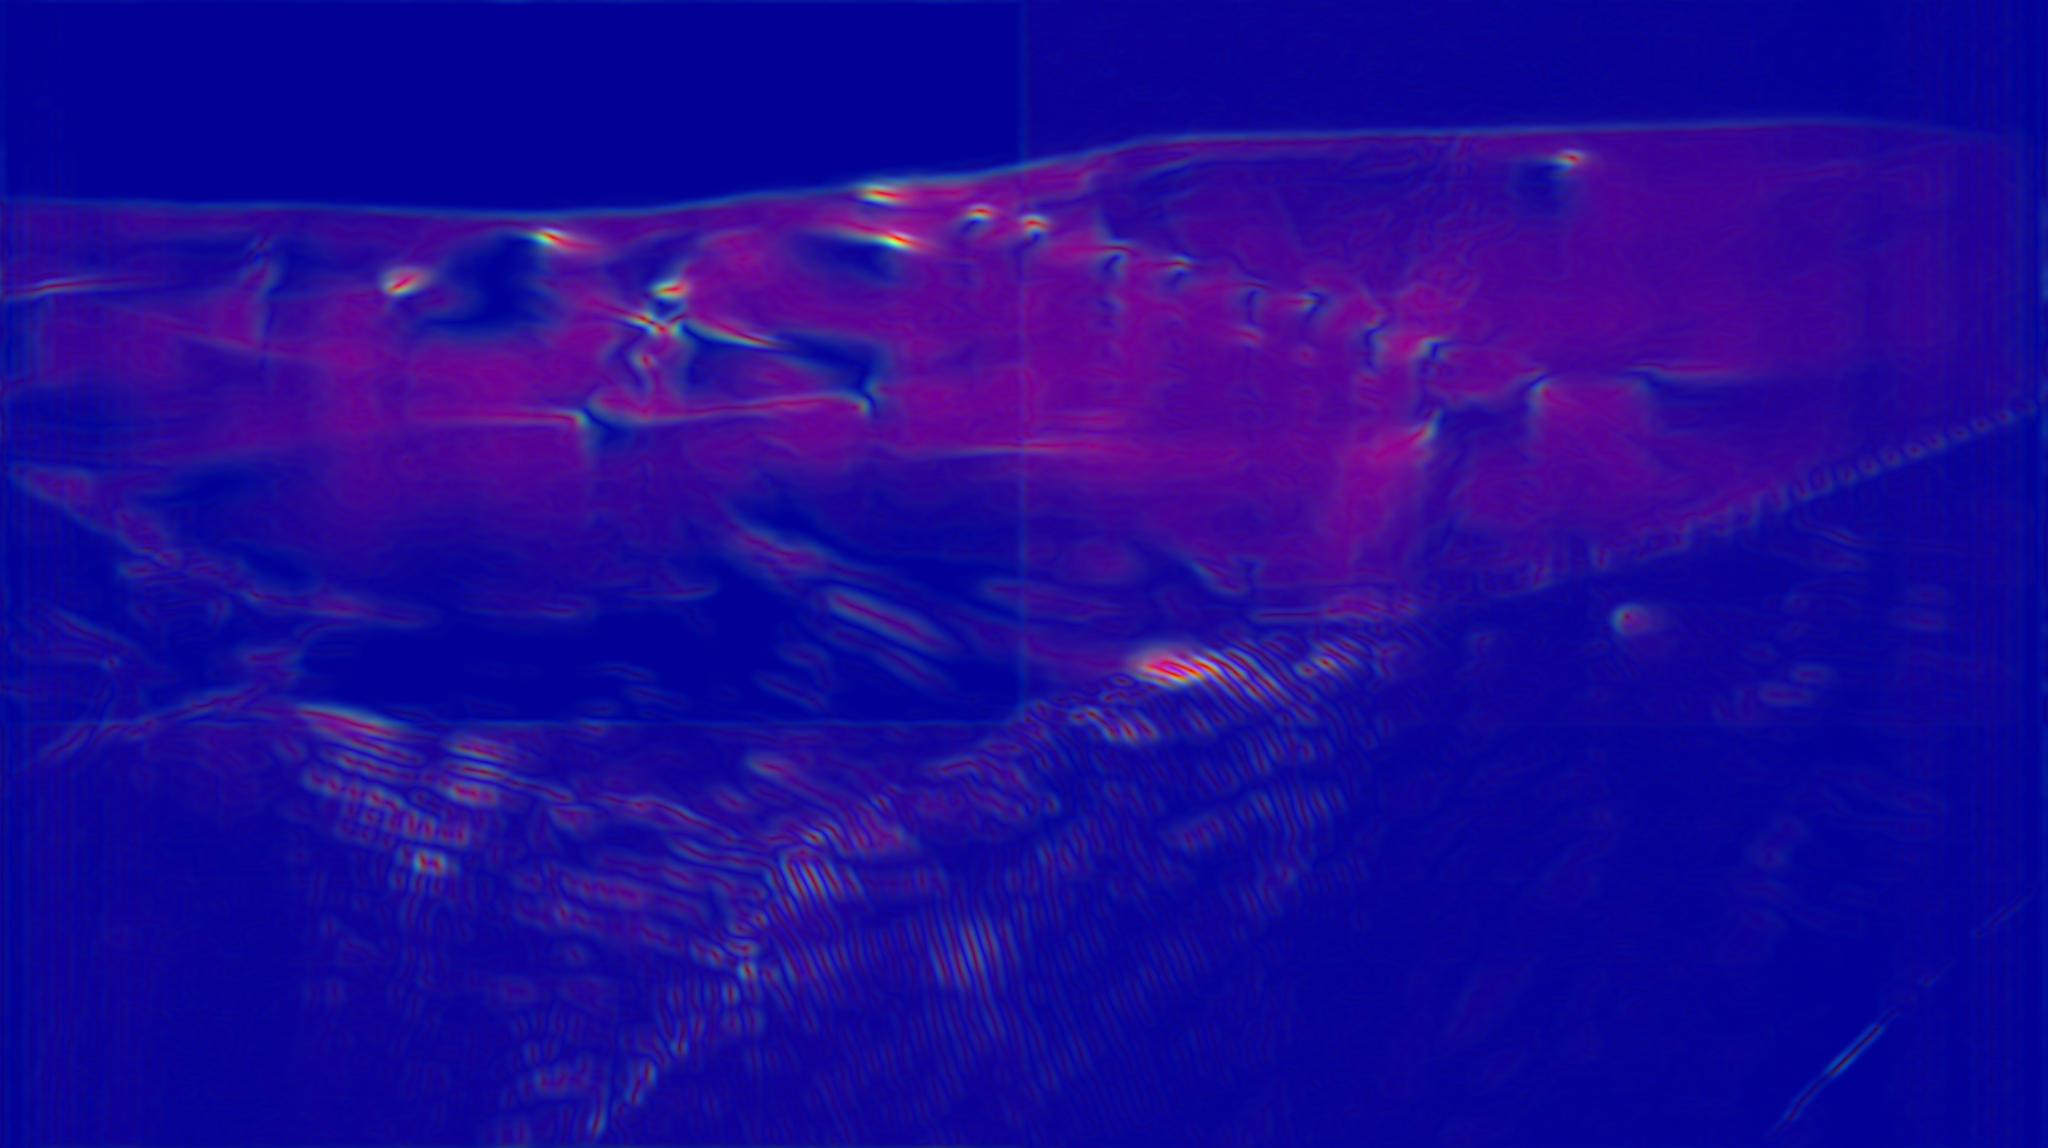
\includegraphics[width=.48\linewidth]{out1_img000}\hfill
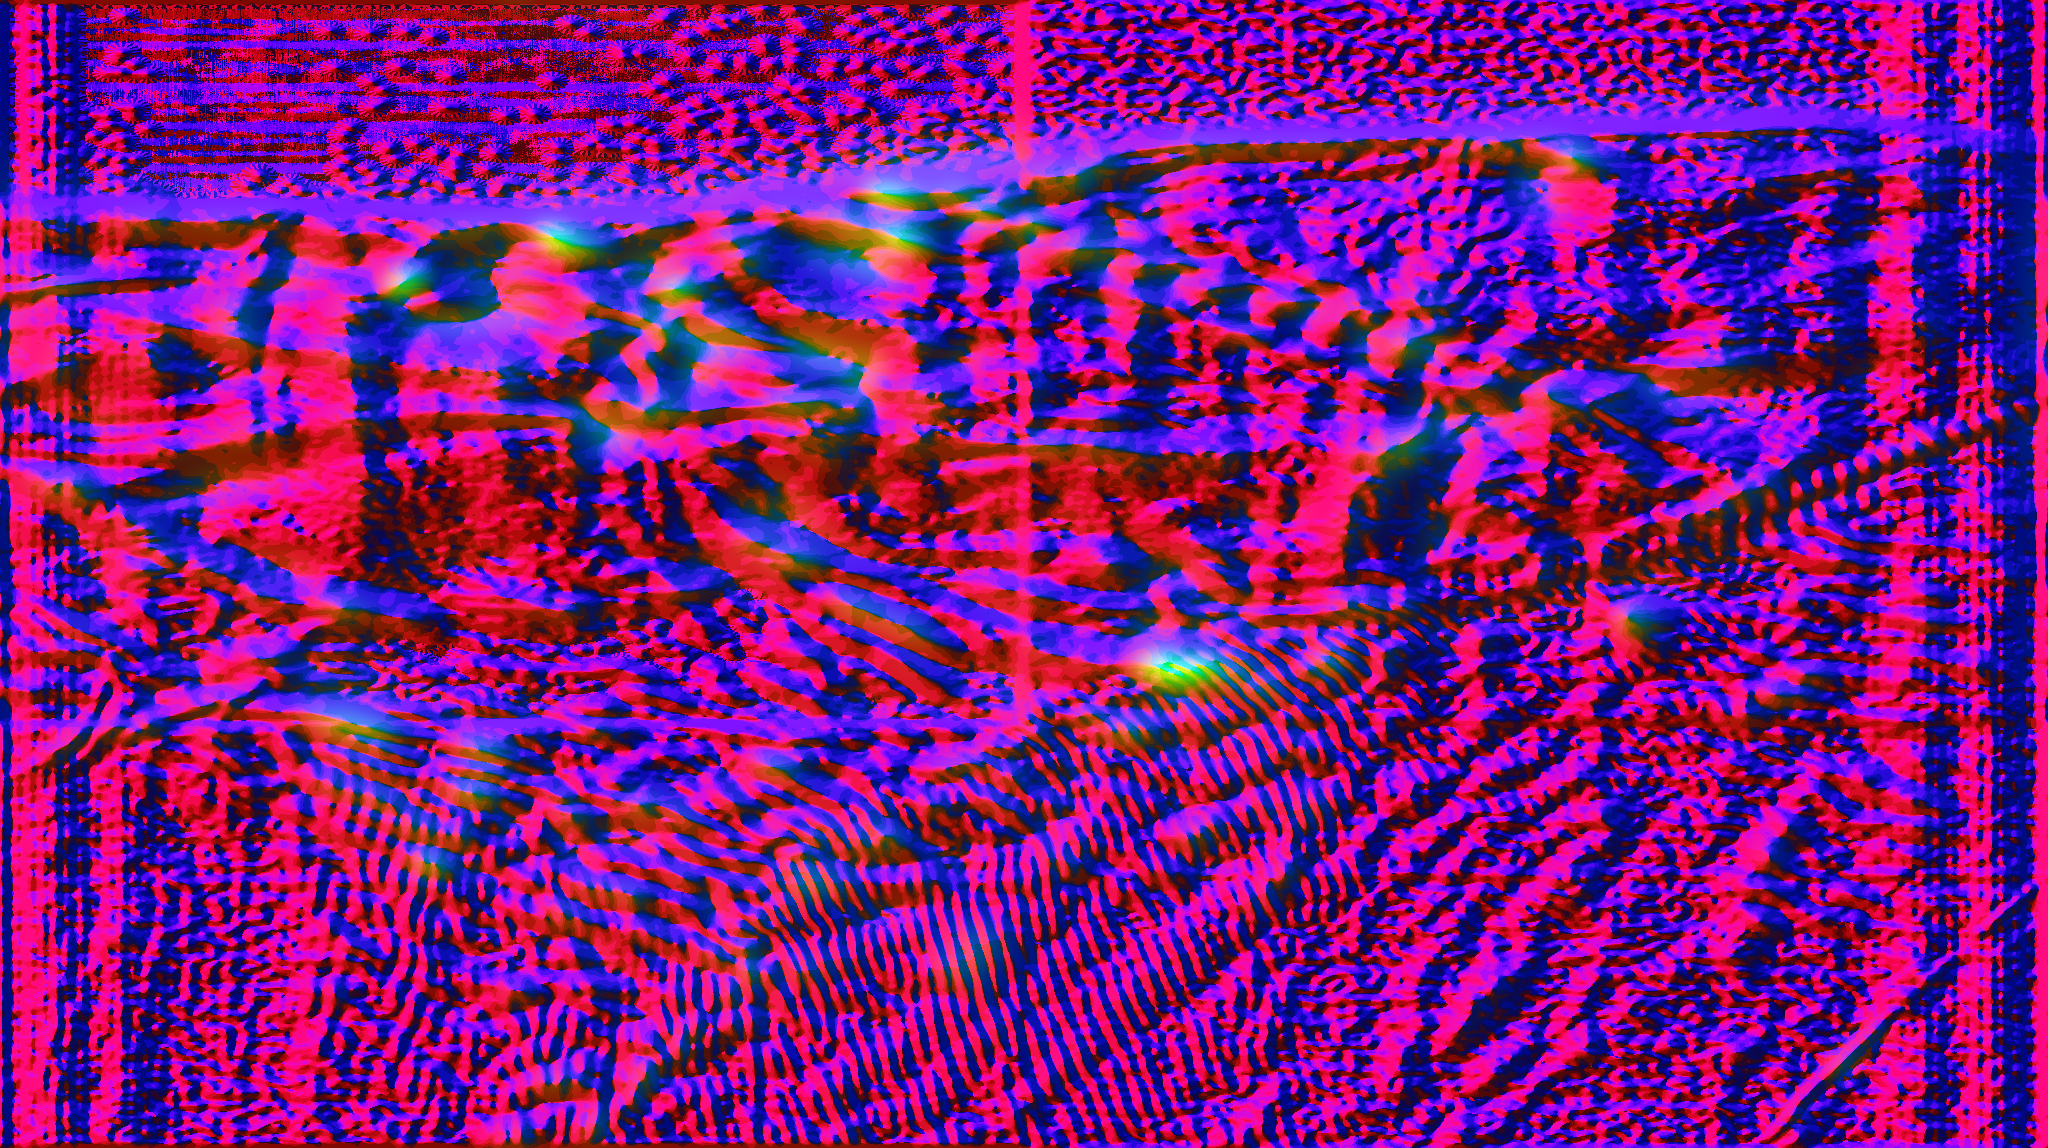
\includegraphics[width=.48\linewidth]{out2_img000}\hfill
}
\end{center}
	We show ``featurization'' results as the three 8-bit color channels in two images.  
	The left color image represents the three features that correspond to an optimal (blue channel), $\nabla^2$ Laplace, and $|\vec{\nabla}|$ filtering with the filter kernels shown at top in their respective color channels.
	The right color image shows the cosine and sine of $\vec{\nabla}/|\nabla|$ as red and blue respectively and the standard deviation filter as the green color channel.
	These features are expected to characterize the local topology of the monochrome original image that would be more suitable for multi-channel matrix input for a convolutional neural network.
	We note that the featurization itself can be represented as fixed convolutional layer with 6 filter channels that would be appropriately flashed to the FPGA chip on the detector.
\end{minipage}%
%}{\begin{minipage}[t]{0.2\linewidth}Ryan, we need words here to describe what was done to create this image that enhances the pearls. Also, I have no idea why this text is beginning at the bottom of the image...\end{minipage}%
}
\hfill
{
\begin{minipage}[t]{0.48\linewidth}
\begin{center}
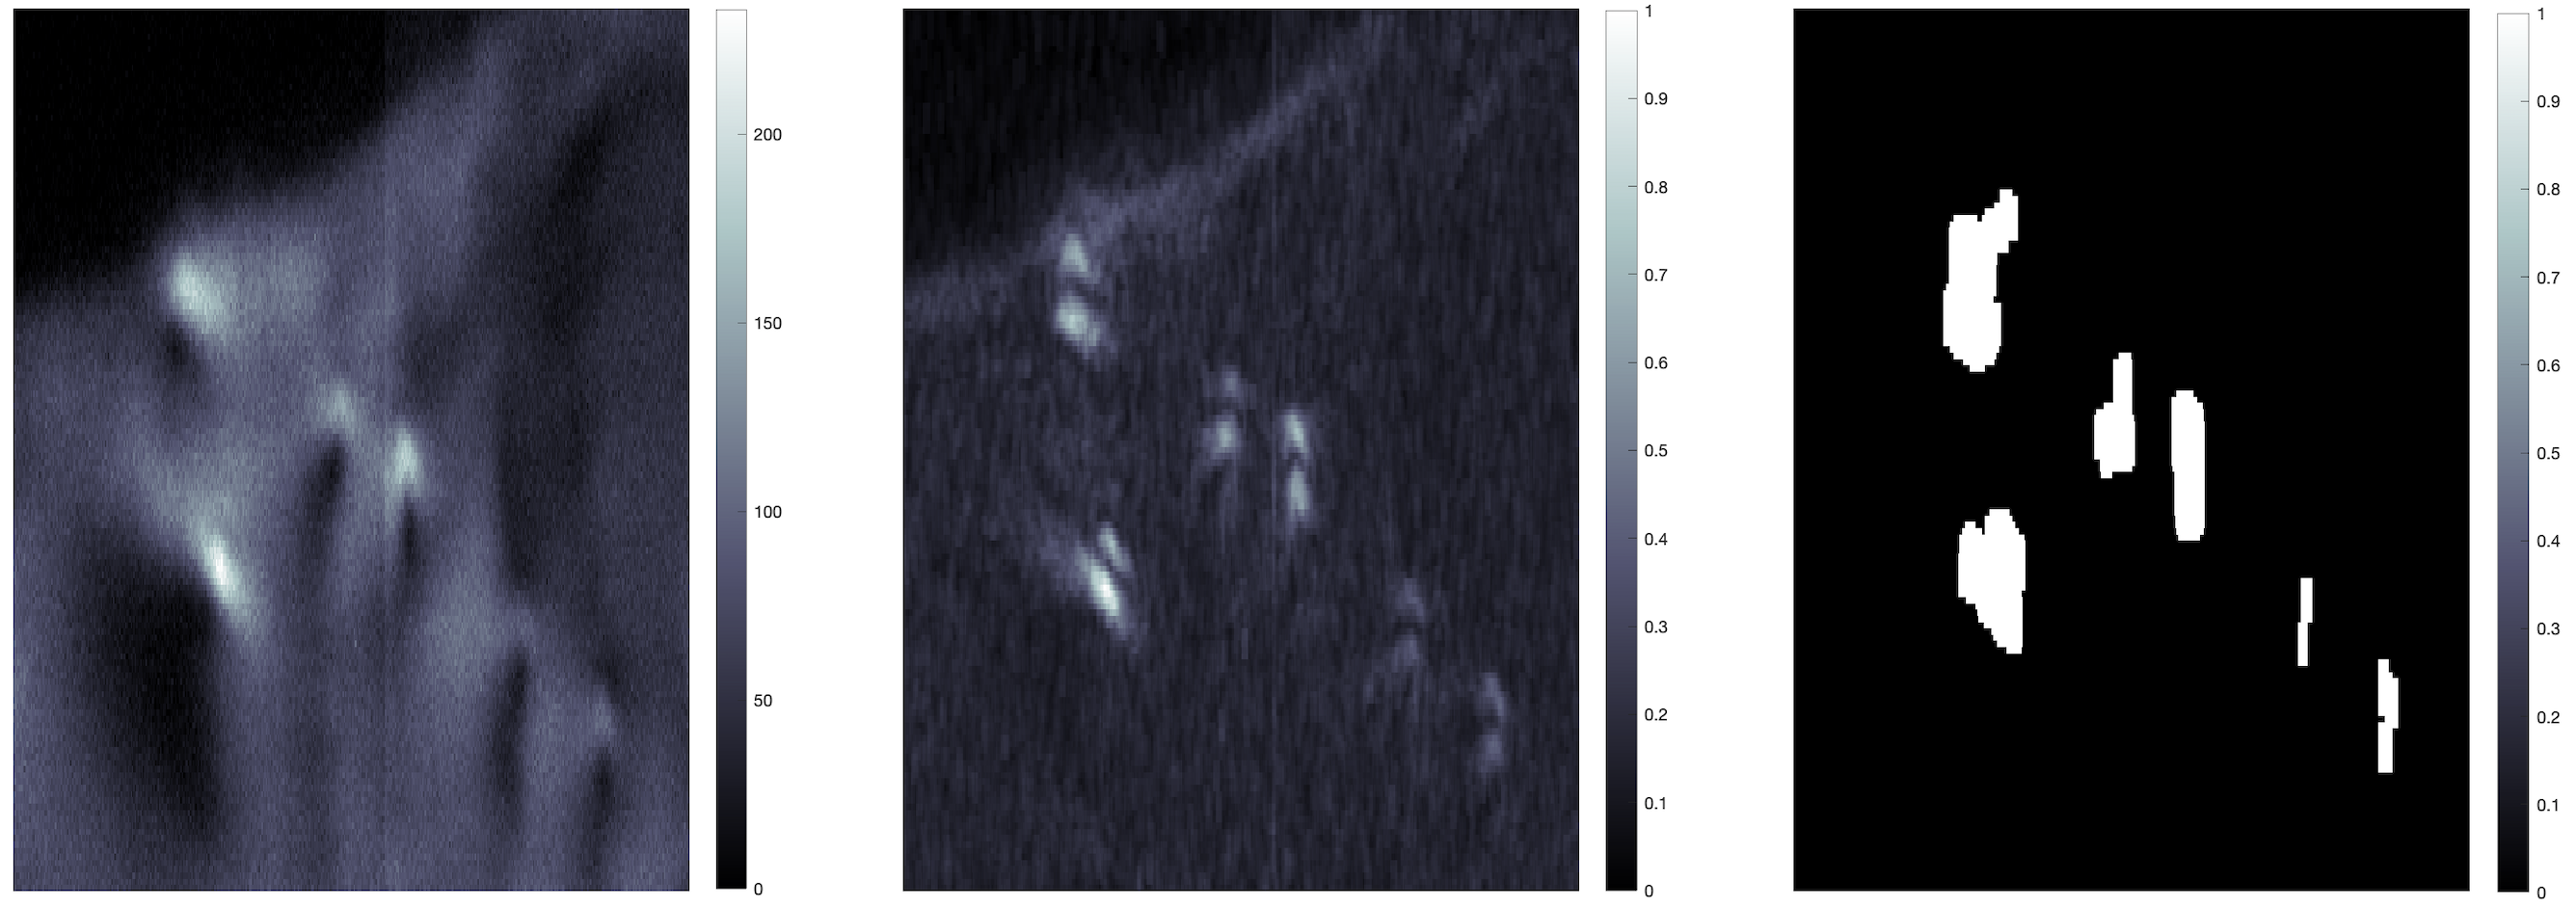
\includegraphics[width=1\linewidth]{sdfilterimages}\end{center}
The original image reduced to a region of interest around the inserting dislocation (left). A standard deviation filter of size 5x5 was convolved across the image (middle). After applying a threshold, the dislocation dark/bright pairs are identified (right).
\end{minipage}
}
\vspace{.2in}

Applying a 2D stationary wavelet transform to the image assists in identification of the dislocation dark/bright pairs, as well in locations where the contrast between dark and bright is not as strong.

{
\begin{minipage}[t]{0.48\linewidth}
\begin{center}
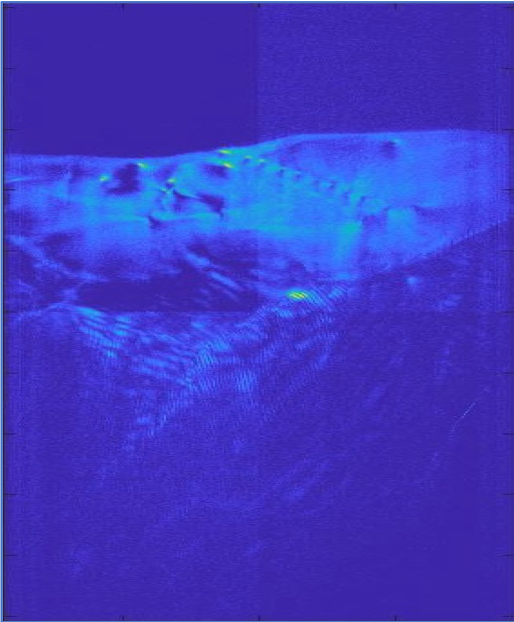
\includegraphics[width=.25\textwidth]{original}
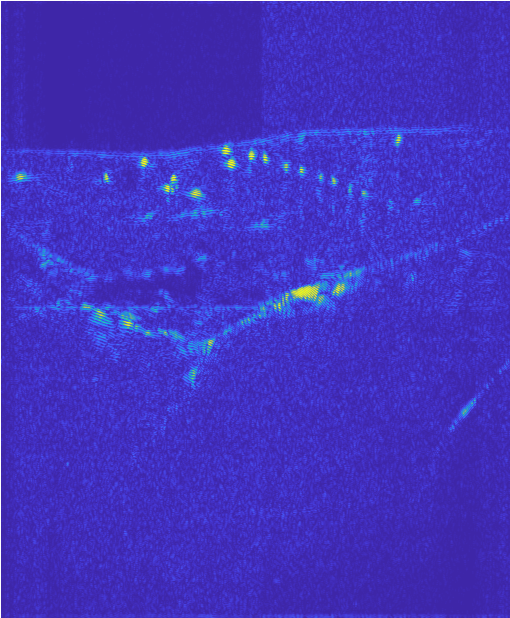
\includegraphics[width=.25\textwidth]{wavelet}
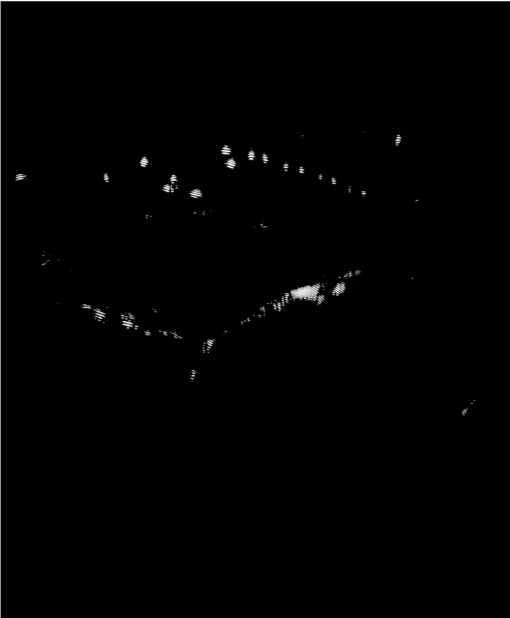
\includegraphics[width=.25\textwidth]{binary}\end{center}
The full, raw image data for one observation in time (left) with its wavelet decomposition (middle). A threshold of the wavelet image (right) lends to identifying and enumerating the dislocations.
\end{minipage}
}{
\begin{minipage}[t]{0.48\linewidth}
\begin{center}
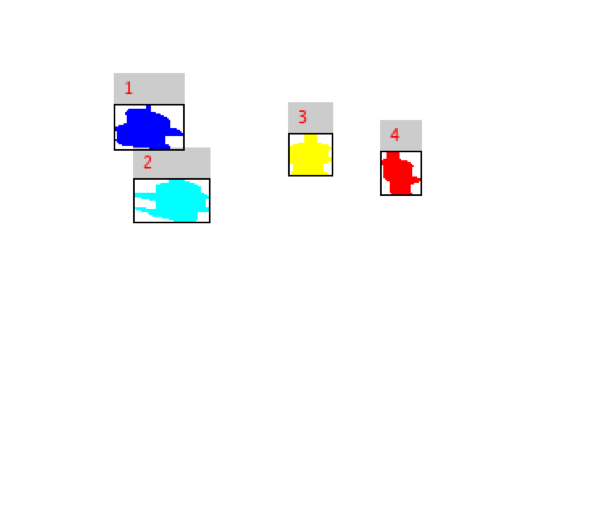
\includegraphics[width=.23\textwidth]{numbereddislocations}
\end{center}
The wavelet analysis with threshold zoomed in to a smaller region of interest, similar to images above. Features and motion of the dislocations can be tracked in time to include statistics such as orientation, velocities, angular velocities, accelerations, and correlations of the velocities.

\end{minipage}
}

{
\begin{center}
%\footnotesize
\begin{tabular}{c|c|c|c|c|c|c} 
%\hline
%\rowcolor{lightgray}
Defect & Avg.  Vel. & 95\% C.I. & Avg. Accel. & 95\% C.I. & Avg. Ang. Vel.  & 95\% C.I.   \\
\hline
1 & 1.29 & [1.14, 1.44]  & 0.006  & [-0.721, 0.700] & 0.70 &[-7.91, 9.40]\\ 
%\hline

2 & 1.95   & [1.59, 2.31] &  -0.064    &  [-1.885, 1.741]  & 0.61  &  [-44.05, 44.86] \\ 
%\hline
3 & 1.68    &   [1.35, 2.11]   &  -0.146    &  [-1.887, 1.569]   & -5.19 & [-33.70, 26.14]   \\
%\hline

4 & 1.57 &  [1.37, 1.84]  & -0.105    &  [-1.229, 1.162] &  4.31   &[ -38.78, 51.16]  \\
%\hline

\end{tabular}
\end{center}
}

%
%\begin{center}
%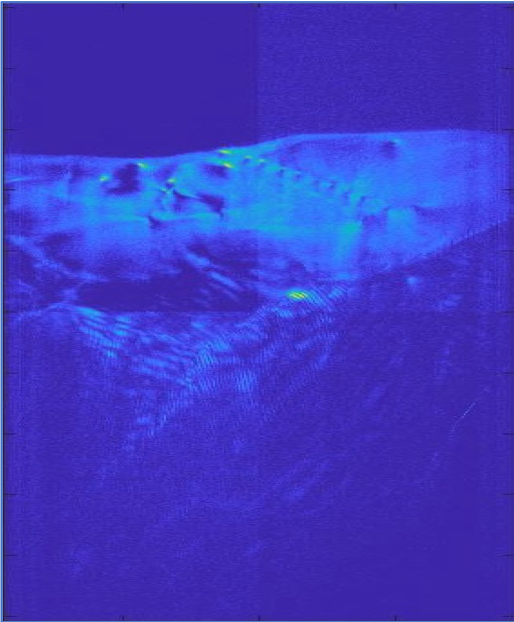
\includegraphics[width=.15\textwidth]{original}
%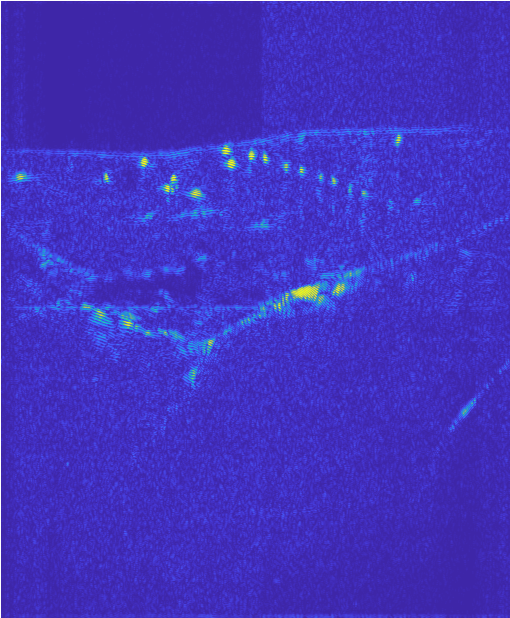
\includegraphics[width=.15\textwidth]{wavelet}
%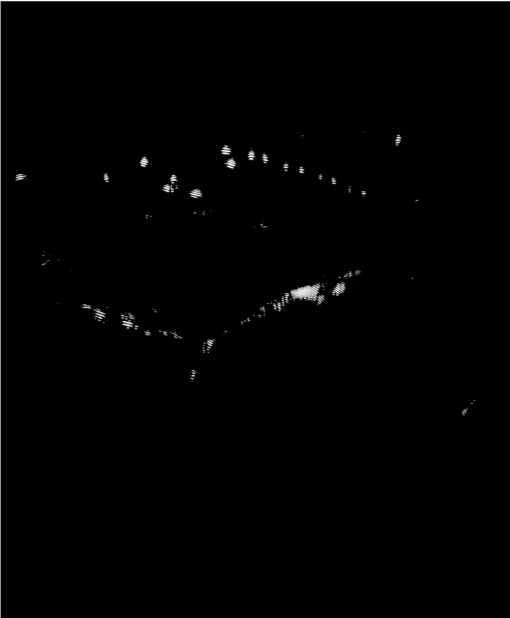
\includegraphics[width=.15\textwidth]{binary} \end{center}
%
%The full, raw image data for one observation in time (first) with its wavelet decomposition (second). A threshold of the wavelet image (third) lends to identifying and enumerating the dislocations.
%------------------------------------------------
}





%----------------------------------------------------------------------------------------
%	ACKNOWLEDGEMENTS
%----------------------------------------------------------------------------------------

\headerbox{Acknowledgements}{name=acknowledgements,column=3,below=experiments, above=bottom}{

\smaller % Reduce the font size in this block
This work was done in part by by Mission Support and Test Services, LLC, under Contract No. DE-NA0003624 with the U.S. Department of Energy and supported by the Site-Directed Research and Development Program. DOE/NV/03624-{}-\\

Who else would like acknowledgements here? \\

This work resulted from the Data Analysis for Nuclear Security Science Workshop 2020.

\begin{center}

\includegraphics[height=0.4in,valign=c]{nnss}\hspace{.2in}
\includegraphics[height=0.4in,valign=c]{llnl}\\
\vspace{0.05in}


\includegraphics[height=0.3in,valign=c]{slac}\hspace{.2in}
\includegraphics[height=0.4in,valign=c]{pnnl}\\
\vspace{0.05in}


\includegraphics[height=0.5in,valign=c]{asu}\hspace{.2in}
\includegraphics[height=0.25in,valign=c]{ua}\hspace{0.2in}
\includegraphics[height=0.3in,valign=c]{mit}
\end{center}
 }
%----------------------------------------------------------------------------------------

\end{poster}

\end{document}
